\documentclass[a4paper,11pt]{article}
\usepackage{graphicx}
\usepackage[T1]{fontenc} % codifica dei font in uscita
\usepackage[utf8]{inputenc} % lettere accentate da tastiera
\usepackage[italian]{babel} % lingua principale del documento
\usepackage{url}
\usepackage [a4paper, top=2.5cm, bottom=2.5cm, left=1.5cm, right=1.5cm, bindingoffset=8mm] {geometry}

% inizio documento
             
\begin{document}

\begin{center}



\textsc{\Huge Esperienza II}\\[0.5cm]



\large
\title{ESPERIENZA IV}

Michele \textsc{Pedrotti}\\
Luigi \textsc{Bassini}\\
Nicola \textsc{Trevisson}\\


\end{center}
\vspace{0.1 cm}
\section{Scopo dell'esperienza}
Lo scopo di questa seconda esperienza è quello di misurare l'apertura numerica della fibra ottica in dotazione. Parallelamente l'esperienza mostra la difficoltà di esecuzione di determinati esperimenti.

\section{Misura dell'apertura numerica di una fibra ottica}
\subsection{Struttura di una fibra ottica}
La Fibra Ottica, che si presenta come un sottile filo di vetro, è costituita da un nucleo cilindrico (core) di un materiale trasparente, circondato da un mantello concentrico (cladding).La fibra è poi protetta esternamente da un rivestimento, in genere realizzato con materiale plastico, per la protezione dalle abrasioni.

 \begin{center} 
\begin{figure}[htpd]
\hspace{90 pt}
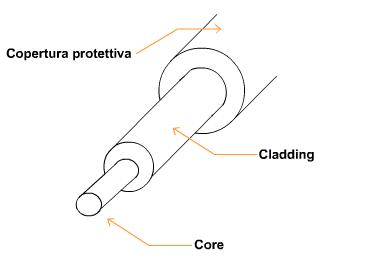
\includegraphics[scale=0.90]{fibre_ottiche.jpg}


\end{figure}
\end{center}

La fibra ottica funziona come una specie di specchio tubolare. La luce che entra nel core entro un certo angolo (angolo limite) si propaga mediante una serie di riflessioni sulla superficie di separazione fra i due materiali del core e del cladding.

 \begin{center} 
\begin{figure}[htpd]
\hspace{90 pt}
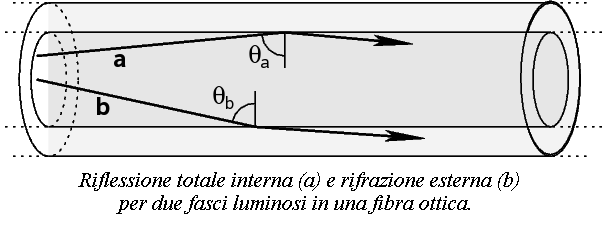
\includegraphics[scale=0.90]{Fibra_ottica2.png}


\end{figure}
\end{center}

Come mostrato in figura, se una radiazione elettromagnetica collide sulla superficie di separazione tra core e cladding con un angolo $\theta \textless \theta \ped{max}$, essa si propaga all'interno della fibra ottica. Al contrario, se essa 
collide sulla superficie di separazione con un angolo $\theta \textgreater \theta \ped{max}$, la radiazione viene rifratta all'esterno del core. 
\subsection{Calcolo dell'apertura numerica}
Il nostro apparato sperimentale consisteva in un laser nella lunghezza d'onda del rosso. Il raggio di tale laser veniva concentrato mediante una lente convergente sulla superficie di uno dei capi della fibra ottica. L'utilizzo della lente convergente è dovuta al fatto che il fascio luminoso possiede un diamotro maggiore rispetto a quello della fibra ottica. Tale capo della fibra ottica era montato su un carrello rotante dotato di goniometro. In questo modo, ruotando il carrello, era possibile variare l'inclinazione della superficie della fibra esposta ai raggi, e di conseguenza la percentuale dei fasci rifratti nel cladding. Per quantificare tale variazione all'alto capo della fibra era posto un fotodiodo, in grado di misurare la potenza della radiazione luminosa. \\
Il nostro obiettivo è quello di misurare l'apertura numerica NA, tramite la relazione: $$NA=n\ped{i}\cdot sin(\theta \ped{max}) $$  
Poichè il nostro esperimento è stato condotto a condizioni ambientali standard n$\ped{i}$=$n\ped{aria}$ $\simeq 1$. La conoscenza dell'apertura numerica è importante in quanto ci consente di conoscere un valore dell'angolo massimo affinchè le onde elettromagnetiche siano completamente riflesse all'interno del core. 
Per prima cosa è stato necessario trovare il valore massimo di potenza passante per la fibra. Questo è stato possibile mediante il cambiamento dell'angolo di inclinazione del carrello su cui era montata l'estremità della fibra esposta al laser. Questo ci ha permesso di notare come l'angolo migliore di esposizione al laser non era $ 0 $ (laser perpendicolare al capo della fibra) ma $ +1.25 $ con un valore di potenza misurato pari a 16$ \mu W $. L'angolazione differente da 0 può essere ricondotta a vari fattori: il non perfetto posizionamento della fibra o del laser sul loro supporto o anche il metoto con cui è stata tagliata la fibra. La sua superfice infatti può non essere regolare e presentare creste e scanalature dovute almetodo di taglio che influenzano più o meno l'ingresso della luce all'interno del core.
Considerando questo valore come il nostro 0 abbiamo modificato l'angolo di incidenza dei fronti d'onda del laser sulla fibra.
Visto che le incognite erano due (l'angolo e l'intensità) abbiamo scelto quale usare come riferimento in modo tale da rendere agevole l'aquisizione dei dati. Si è cosi scelto come riferimento il valore di intensità luminosa anziche l'angolo. La variazione costante dell'angolo infatti ci avrebbe impedito di avere una distribuzione regolare dei punti sul grafico.
Di conseguenza la fibra è stata ruotata in modo tale da far diminuire l'intensità di circa $ 1\mu W$ e quando ciò accadeva si rilevava l'angolo corrispondente. Una volta raggiunto il valore minimo di intensità luminosa abbiamo ripetuto la misurazione riportando il carrello sull'angolo iniziale. E' da notare però che dopo il primo set di misurazioni l'angolo di massima esposizione era cambiato.




\end{document}